\subsection{Simulation}

\subsubsection{Aufbau}

\begin{figure}[h!]
	\centering
	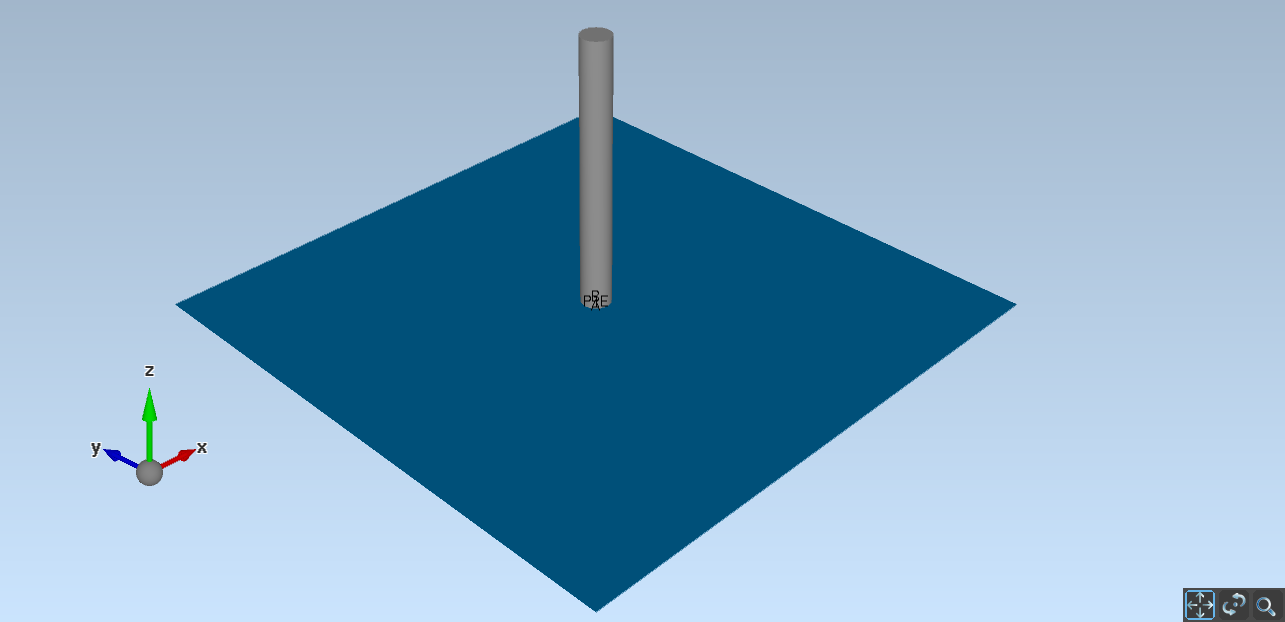
\includegraphics[width=0.75\textwidth]{../fig/plt/monopol_a_sim_3d_model.png}
	\caption{Erstelltes Simulationsmodell.}
\end{figure}

Das Simulationsmodell entspricht der zuvor vorgestellten Geometrie.
Für die Simulation wurde dem Modell noch eine Quelle hinzugefügt,
welche die Einspeisung repräsentiert. Diese ist zwischen dem
Stab und der Groundplane platziert, wodurch diese miteinander
über die Quelle verbunden werden.

\newpage
\subsubsection{Reflexionskoeffizient}

\begin{figure}[h!]
	\centering
	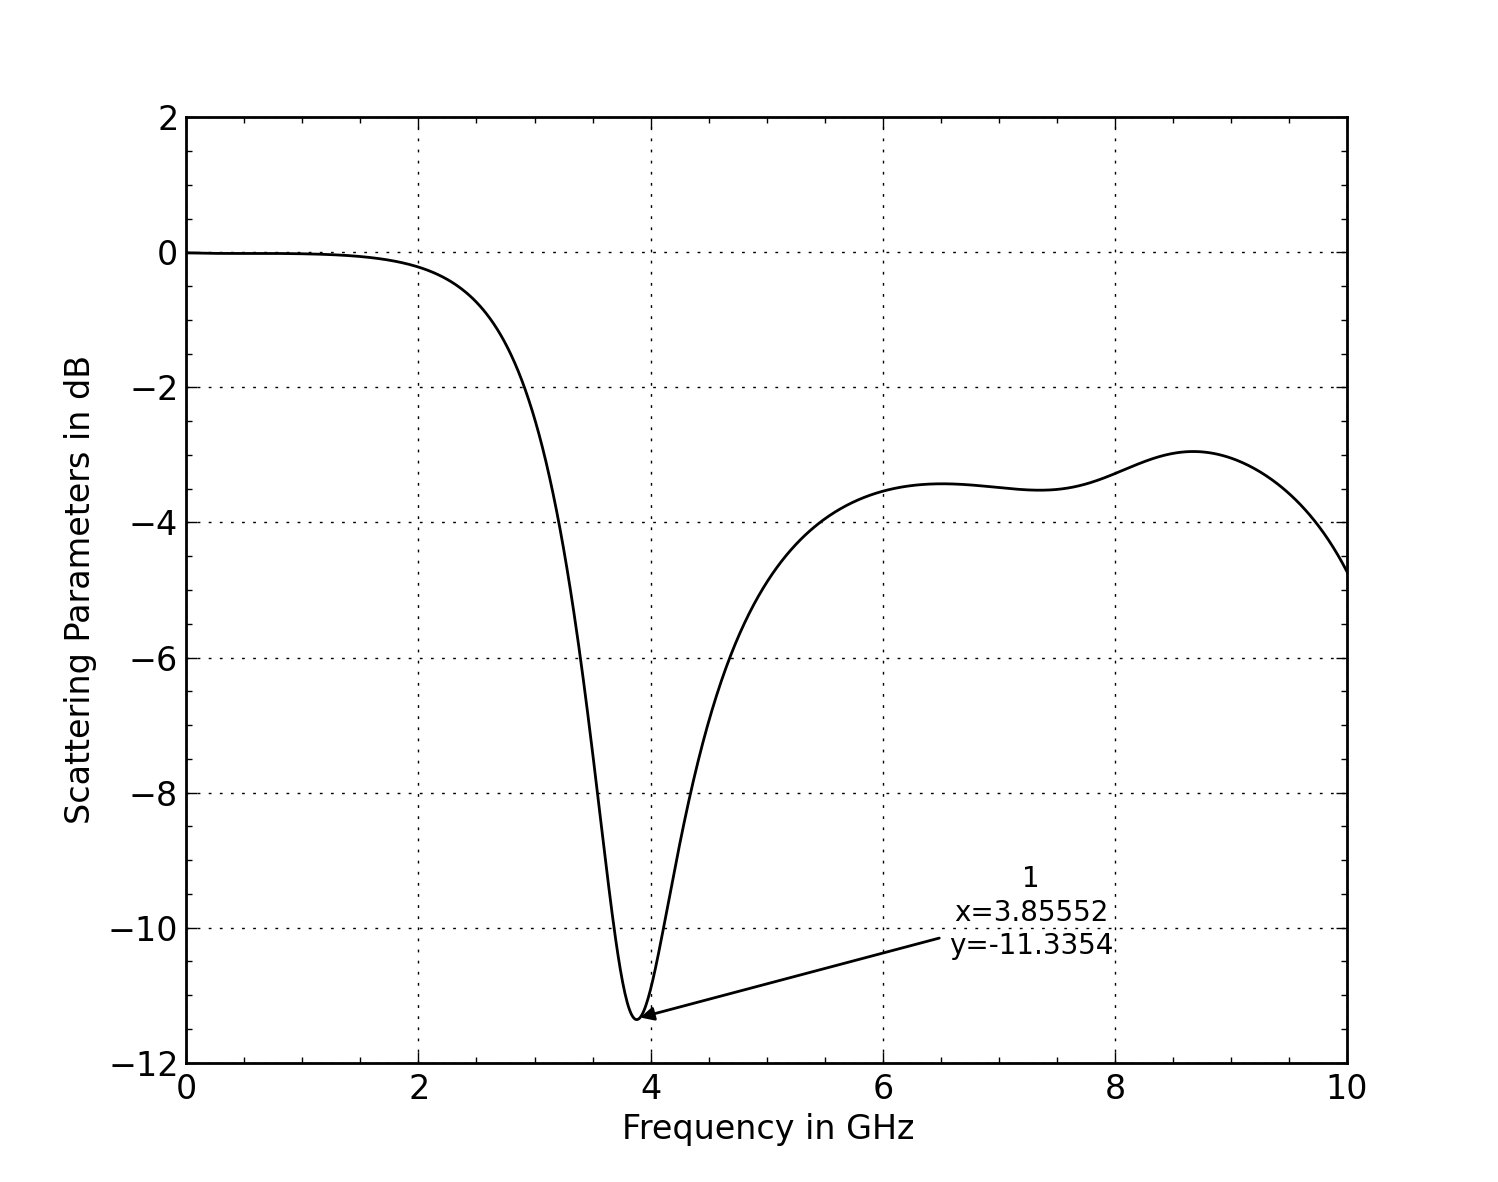
\includegraphics[width=0.75\textwidth]{../fig/plt/monopol_a_sim_s11.png}
	\caption{Reflexionskoeffizient ($S_{11}$ Parameter).}
\end{figure}

Die Simulation zeigt, dass die beste Abstrahlung leicht unter der
gewünschten Frequenz von \SI{4}{\giga\hertz} liegt. Dieses Ergebnis
kann nun in der Weise interpretiert werden, dass die erstellte
Antenne zu \emph{lang} ist. Durch die Kürzung der Stablänge $l_S$
kann dies korrigiert werden, denn damit wird die Wellenlänge
$\lambda$ reduziert und folglich die Frequenz erhöht.

\newpage
\subsubsection{Antennenimpedanz}

\begin{figure}[h!]
	\centering
	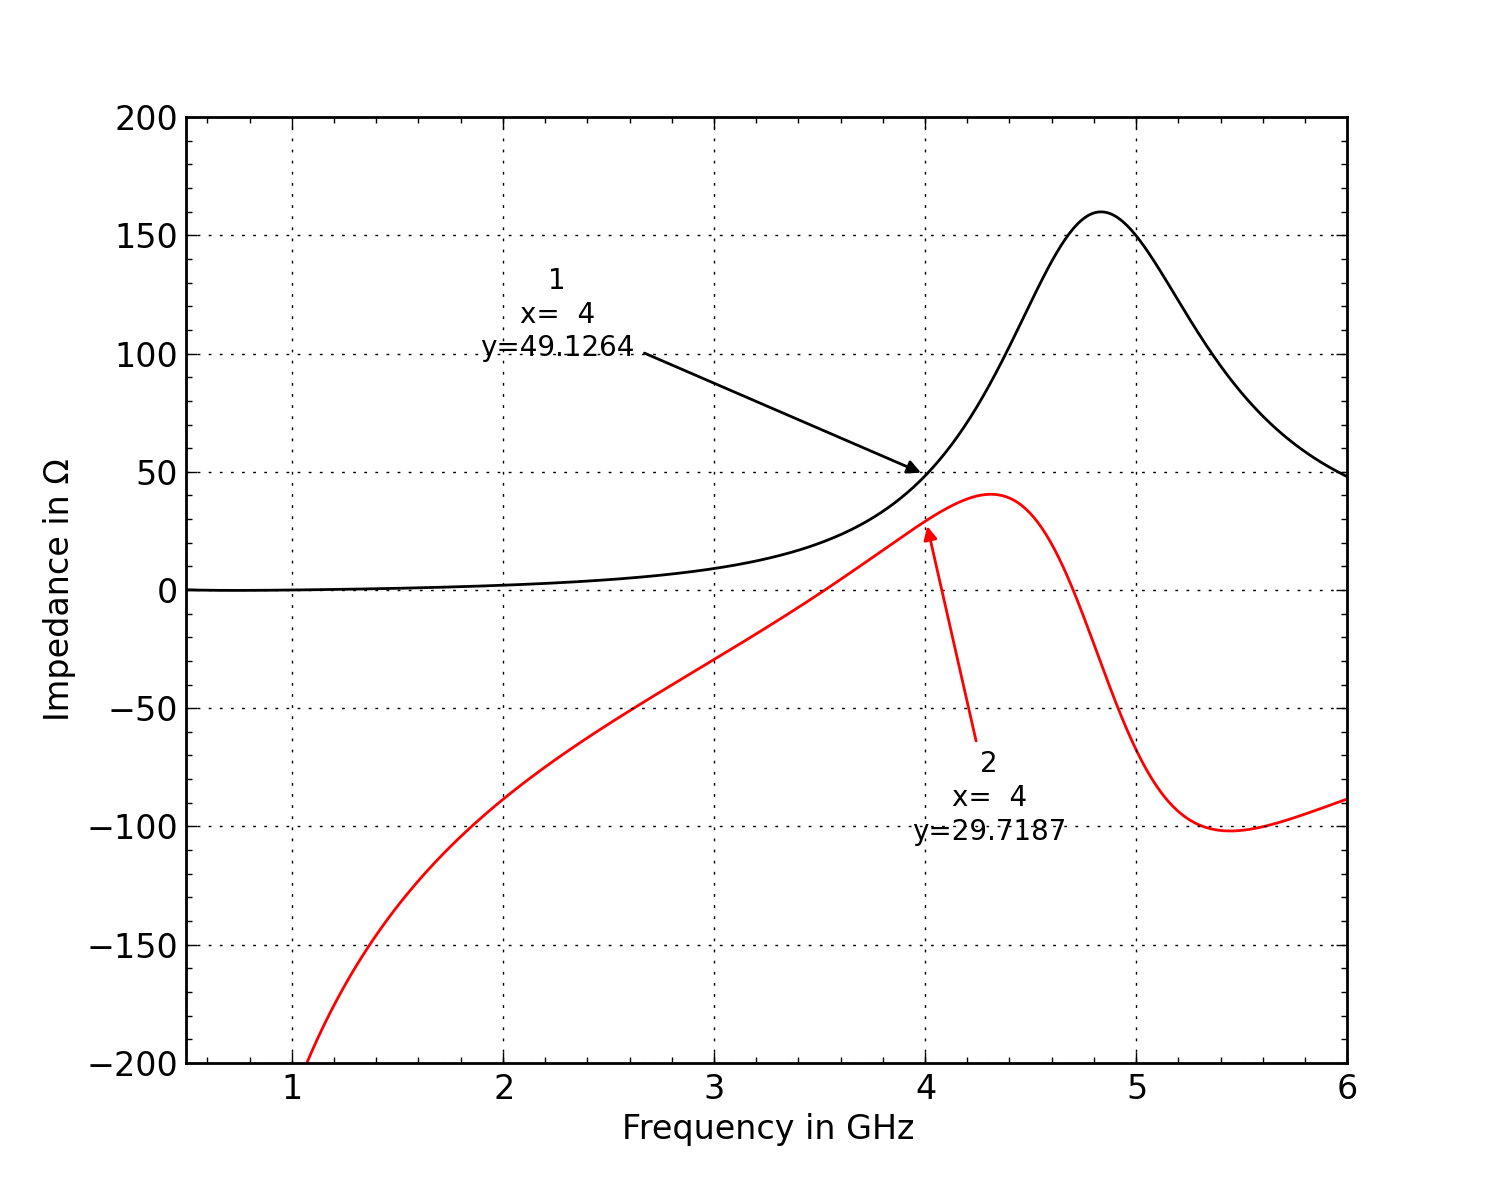
\includegraphics[width=0.75\textwidth]{../fig/plt/monopol_a_sim_impedance.png}
	\caption{Antennenimpedanz ($\mathrm{Re}\left\{Z\right\}$ schwarz,  $\mathrm{Im}\left\{Z\right\}$ rot).}
\end{figure}

Die Simulation zeigt, dass der Realanteil
$\mathrm{Re}\left\{Z\right\} \approx \SI{50}{\ohm}$ und somit dem
gewünschten Wert entspricht. Der Imaginäranteil ist mit
$\mathrm{Im}\left\{Z\right\} \approx \SI{30}{\ohm}$ deutlich über
dem geforderten Wert von \SI{0}{\ohm}, hat induktiven Charakter (da
$\mathrm{Im}\left\{Z\right\} > 0$) und bedeutet, dass eine suboptimale
Ausnutzung vorliegt (da ein Teil der Leistung nicht abstrahlungsfähig
ist durch die resultierende Reflexion). Weiter ist in der Abbildung ein
nahe liegener Resonanzpunkt zu erkennen bei ca. \SI{4.8}{\giga\hertz}.
Da dieser Resonanzpunkt nahe liegt und die Impedanz in dessen Umgebung
eine hohe Änderungsrate $\frac{\mathrm{d}Z}{\mathrm{d}f}$ besitzt,
bedeutet dies, dass die Impedanzverhältnisse nicht robust und die
Antenne \emph{empfindlich} ist auf eine Änderung der Frequenz $f$.
Die Simulation zeigt, dass eine Änderung der Frequenz um 
\SI{400}{\mega\hertz} den Realanteil der Impedanz bereits
verdoppelt auf \SI{100}{\ohm}.


\newpage
\subsubsection{2D Richtdiagramm}

\begin{figure}[h!]
	\centering
	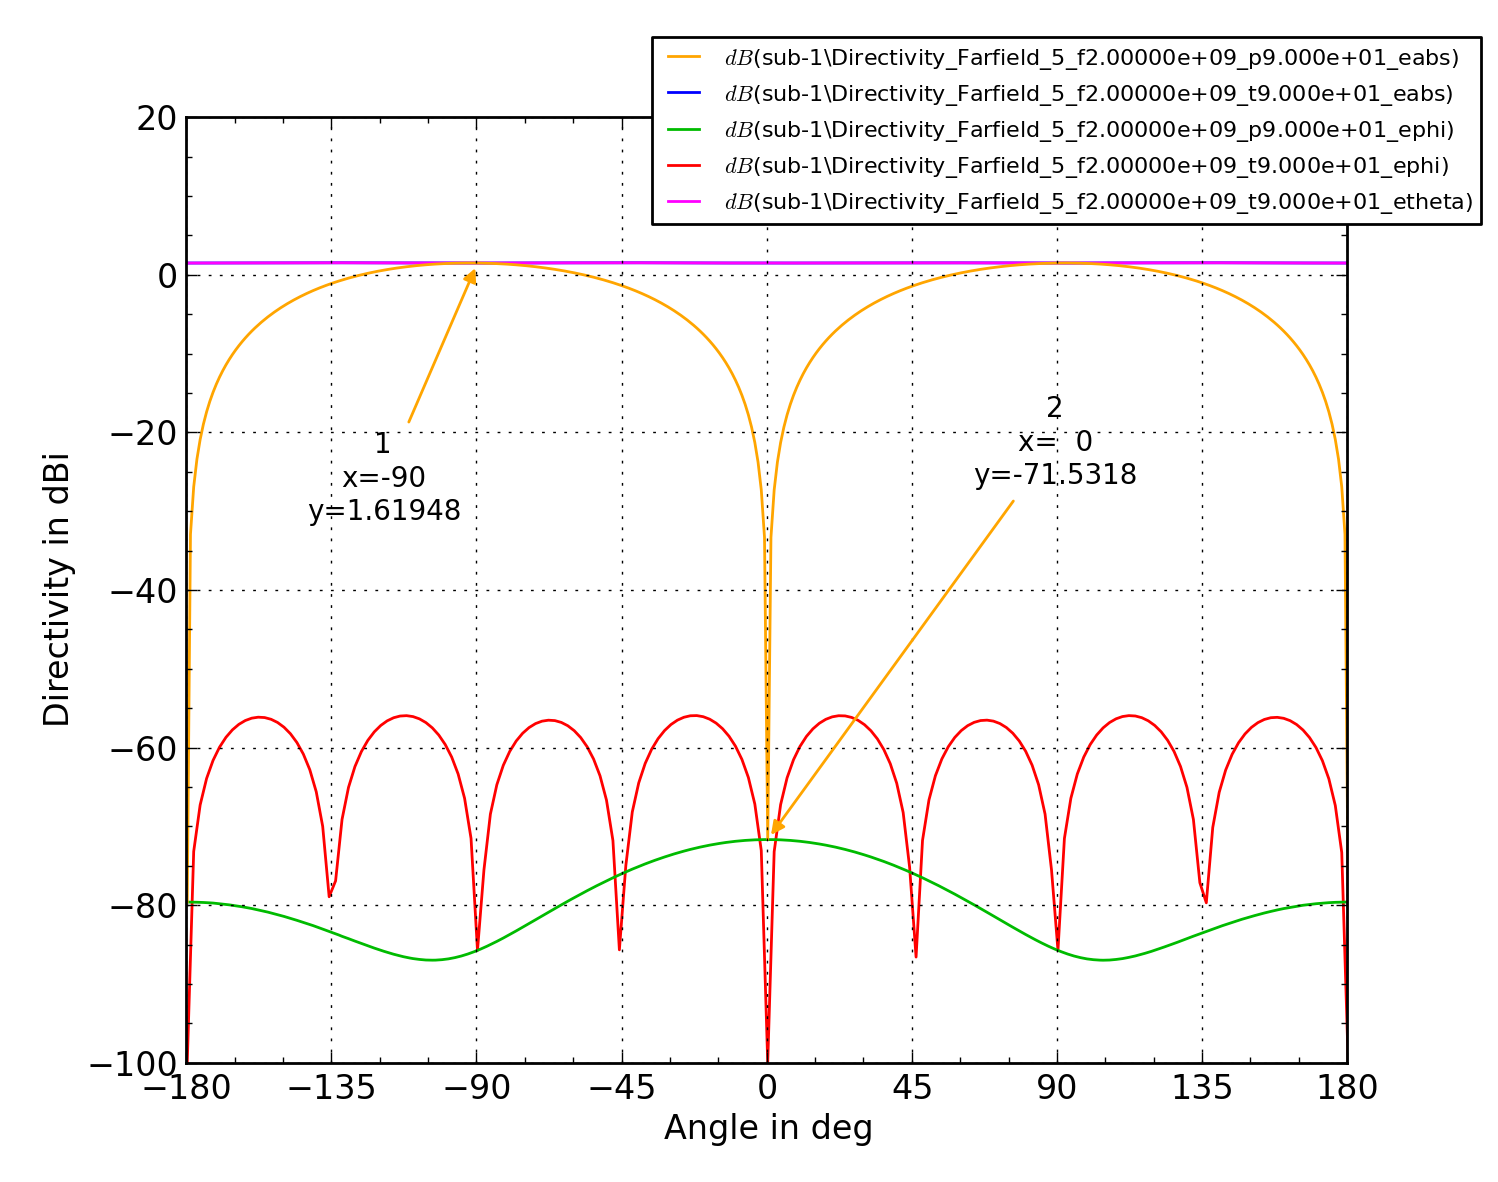
\includegraphics[width=0.75\textwidth]{../fig/plt/monopol_a_sim_2d_pattern.png}
	\caption{2D Richtdiagramm.}
\end{figure}

Die Simulation zeigt, dass die Antenne die erwatrete Abstrahlcharakteristik
eines idealen Monopols aufweist, welcher eine maximale Abstrahlung bei
$\pm \SI{90}{\degree}$ (senkrecht zum Stab) und die minimale Abstrahlung
bei \SI{0}{\degree} respektive \SI{180}{\degree} (entland des Stabs)
aufweist ($E_{\mathrm{abs}}$).

\newpage
\subsubsection{3D Richtdiagramm}

\begin{figure}[h!]
	\centering
	%\begin{subfigure}[b]{0.48\textwidth}
		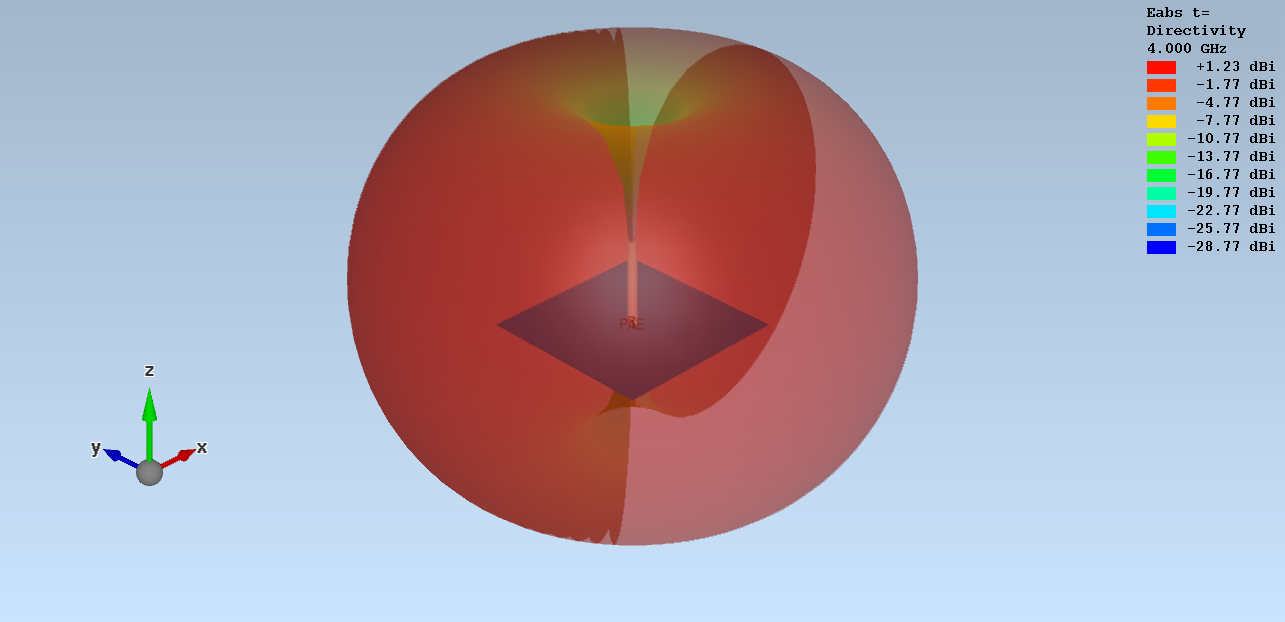
\includegraphics[width=1\textwidth]{../fig/plt/monopol_a_sim_3d_eabs.png}
	%	\caption{E-Feld Absolut}
	%\end{subfigure}
	%\begin{subfigure}[b]{0.48\textwidth}
	%	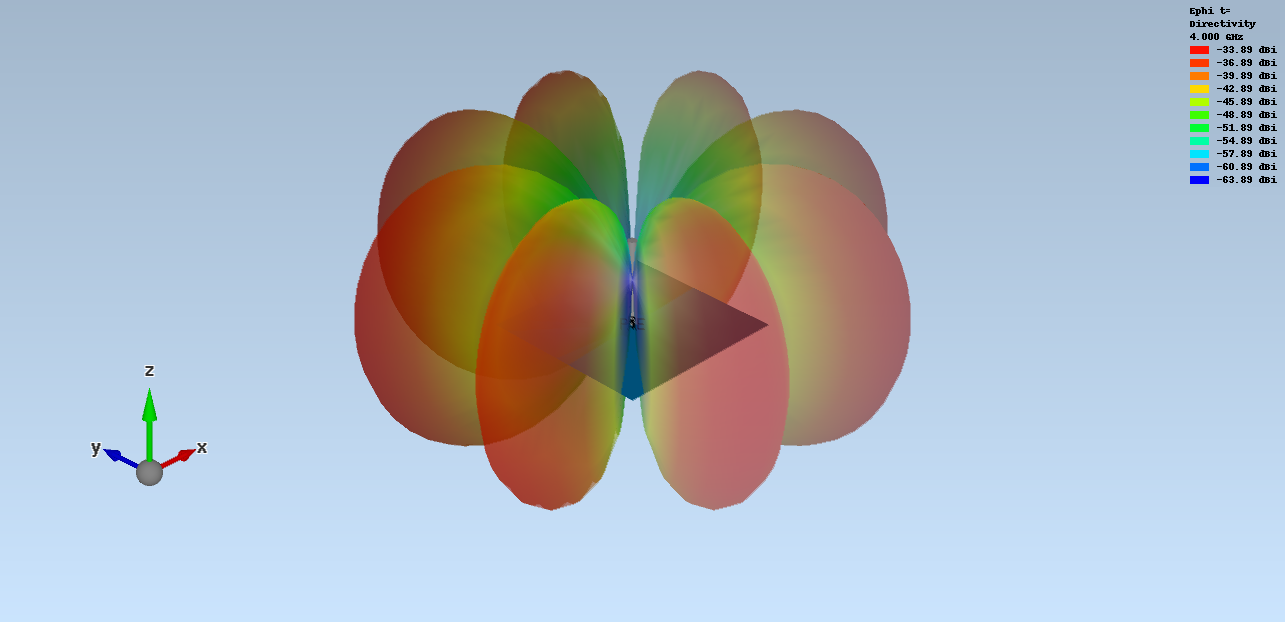
\includegraphics[width=1\textwidth]{../fig/plt/monopol_a_sim_3d_ephi.png}
	%	\caption{E-Feld $\varphi$}
	%\end{subfigure}
	\caption{3D Darstellung des Fernfeldes}
\end{figure}

Die Simulation zeigt wie bereits das 2D Richtdiagramm die Abstrahlung
der Antenne ($E_{\mathrm{abs}}$). Hier ist nochmals deutlich zu sehen,
dass die Antenne \emph{seitwärts} gut abstrahlt, \emph{auf-} und
\emph{abwärts} jedoch ein \emph{Funkloch} besteht.
